\paragraph{\trBraidGroup{}与\trMappingClassGroup。}\label{sub:braid-mapping-class}
现在我们专门讨论最简单的非形式情形 $n=1$、$m=5$，并从一个不同的角度来考察这一局面——这个角度解释了高阶\trComposition{}映射的几何意义。把 \eqref{eq:tw-quasi-equivalence} 的\trEquivalence{}与\trYonedaEmbedding{}结合起来，便得到一个\trFullyFaithful{}的\trAFunctor
\begin{equation}\label{eq:yoneda-functor}
\scr{F}(X)\longrightarrow\scr{Q}=\mathit{mod}(\scr{F}).
\end{equation}
它把一个\trExactLagrangianBrane{}$L^\#$ 送到一个\trAinfty-模 $\scr{M}$，后者的\trCohomology{}是 $M=H(\scr{M})=\bigoplus_i HF^*(V_i^\#,L^\#)$，被看成 $A=\bigoplus_{i,j}HF^*(V_i^\#,V_j^\#)$ 上的一个\trModule。我们将特别关注\cref{fig:curve-l-genus2}中所画的那条曲线 $L$。它具有零\trMaslov{}数，并且可以做成\trExact{}的，因而成为一个\trExactLagrangianBrane。在\trGrading{}的适当选取下，与之相伴的\trModule{}是
\begin{equation*}
M=U_3\oplus SU_3,
\end{equation*}
其中的记号是：$U_i=(i)R\cong\KK$ 为诸初等单模（$R$ 作为 $A$ 上右模的诸\trDirectSummand），而 $S$ 照例指\trSuspension。
\begin{figure}[htbp]
\centering
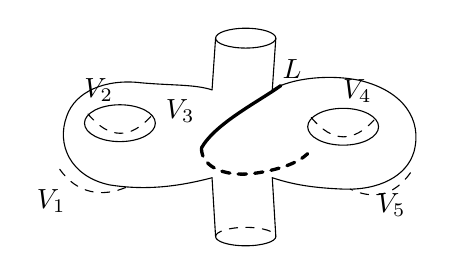
\begin{tikzpicture}[line cap=round,line join=round,scale=0.9]
\draw (0.5,0.62) .. controls (0.75,0.78) and (1.3,0.85) .. (1.75,0.75)
      .. controls (2.35,0.6) and (2.62,0.2) .. (2.5,-0.25)
      .. controls (2.4,-0.6) and (2.0,-0.8) .. (1.5,-0.78)
      .. controls (1.0,-0.76) and (0.75,-0.7) .. (0.5,-0.62);
\draw (-0.35,-0.62) .. controls (-0.85,-0.75) and (-1.3,-0.8) .. (-1.8,-0.72)
      .. controls (-2.35,-0.6) and (-2.55,-0.15) .. (-2.4,0.25)
      .. controls (-2.28,0.6) and (-1.85,0.78) .. (-1.35,0.72)
      .. controls (-0.9,0.68) and (-0.6,0.7) .. (-0.35,0.62);
\draw (0.5,0.62) -- (0.55,1.35);
\draw (-0.35,0.62) -- (-0.3,1.35);
\draw (0.125,1.35) ellipse (0.425 and 0.14);
\draw (0.5,-0.62) -- (0.55,-1.45);
\draw (-0.35,-0.62) -- (-0.3,-1.45);
\draw[dashed] (-0.3,-1.45) arc(180:0:0.425 and 0.13);
\draw (-0.3,-1.45) arc(180:360:0.425 and 0.13);
\draw (-1.65,0.15) ellipse (0.5 and 0.26);
\draw[dashed] (-2.1,0.28) .. controls (-1.8,-0.08) and (-1.5,-0.08) .. (-1.2,0.26);
\draw (1.5,0.1) ellipse (0.5 and 0.26);
\draw[dashed] (1.05,0.23) .. controls (1.35,-0.13) and (1.65,-0.13) .. (1.95,0.21);
\draw[dashed] (-2.5,-0.5) .. controls (-2.25,-0.85) and (-1.9,-0.9) .. (-1.55,-0.75);
\draw[dashed] (2.45,-0.55) .. controls (2.2,-0.9) and (1.9,-0.92) .. (1.6,-0.78);
\draw[very thick] (0.62,0.68) .. controls (0.3,0.45) and (-0.3,0.15) .. (-0.5,-0.2);
\draw[very thick,dashed] (-0.5,-0.2) .. controls (-0.5,-0.5) and (-0.1,-0.62)
      .. (0.3,-0.55) .. controls (0.6,-0.5) and (0.85,-0.42) .. (1.0,-0.28);
\node at (-1.95,0.62) {$V_2$};
\node at (-0.8,0.32) {$V_3$};
\node at (1.7,0.6) {$V_4$};
\node at (-2.62,-0.95) {$V_1$};
\node at (2.18,-1.0) {$V_5$};
\node at (0.78,0.92) {$L$};
\end{tikzpicture}
\caption{}\label{fig:curve-l-genus2}
\end{figure}
我们现在对单模 $U_3$ 的\trHomology{}代数稍作更细致的考察。把诸初等投射模记作 $P_i=(i)A$。有一个\trAcyclic\trComplex
\begin{equation*}
\begin{gathered}
0\to S^{-3}U_3\to S^{-2}P_3\to S^{-1}P_2\oplus S^{-2}P_4\\
\to P_1\oplus S^{-1}P_3\oplus S^{-2}P_5\to P_2\oplus S^{-1}P_4\to P_3\to U_3\to 0,
\end{gathered}
\end{equation*}
它可以循环地衔接起来，构成 $U_3$ 的一个无穷投射分解。利用这一点，可以算出（其中的\trGrading{}记法与\trHochschildCohomology{}群的情形相类比）
\begin{equation}\label{eq:ext-u3-computation}
\begin{aligned}
&\operatorname{Ext}^{r+s}_{A}(U_3,U_3)^s=0\quad\text{每当 } r+s<0\text{ 时；}\\
&\operatorname{Ext}^{0}_{A}(U_3,U_3)^{0}=\KK\text{，而 }
\operatorname{Ext}^{0}_{A}(U_3,U_3)^{s}=0\quad\text{对一切 } s\ne 0\text{；}\\
&\operatorname{Ext}^{1}_{A}(U_3,U_3)^{-1}=\KK\text{，而 }
\operatorname{Ext}^{1}_{A}(U_3,U_3)^{s}=0\quad\text{对一切 } s\ne 1.
\end{aligned}
\end{equation}
最后，知道了这些之后，再使用\trBarResolution——或者代之以与扩大代数 $\bar{A}$ 的类似结果作比较——便可进一步看出，乘积
\begin{equation}\label{eq:ext-product-nonzero}
\operatorname{Ext}^{1}_{A}(U_3,U_3)^{-1}\otimes\operatorname{Ext}^{1}_{A}(U_3,U_3)^{-1}
\longrightarrow\operatorname{Ext}^{2}_{A}(U_3,U_3)^{-2}
\end{equation}
是非零的。这些计算的意义如下。设 $\tilde{\scr{A}}$ 是 $A$ 上的平凡\trAinfty{}结构，并设 $\widetilde{\scr{Q}}=\mathit{mod}(\tilde{\scr{A}})$ 是它的\trAinfty-模\trCategory。有一种普遍的方法，用来对具有固定\trCohomology{}模 $M$ 的 $\tilde{\scr{A}}$-模 $\widetilde{\scr{M}}$ 进行分类，它由\trKodaira--\trSpencer\trDeformation{}理论意义下的 $\operatorname{Ext}^1_A(M,M)$ 所支配。在这一语境中，\eqref{eq:ext-u3-computation} 与 \eqref{eq:ext-product-nonzero} 描述了一个一阶\trDeformation{}为一维、而全体在二阶处受阻的理论。于是，在 $H^0(\widetilde{\scr{Q}})$ 中相差\trIsomorphism{}的意义下，把 $U_3$ 做成 $\tilde{\scr{A}}$-模 $\widetilde{\scr{U}}_3$ 的方式只有一种（即平凡的那一种）。使用同一套形式体系的、略微复杂一些的一个论证（其细节从略）给出如下结论：
\begin{lemma}\label{thm:module-unique-extension}
设 $\widetilde{\scr{M}}$ 是 $\tilde{\scr{A}}$ 上的一个\trAinfty-模，其底\trCohomology{}模为 $H(\widetilde{\scr{M}})\cong U_3\oplus SU_3$。那么
\begin{equation*}
\widetilde{\scr{M}}\cong\scr{C}one(t)\quad\text{在 } H^0(\widetilde{\scr{Q}})\text{ 中，}
\end{equation*}
其中 $t\in\hom^0_{\widetilde{\scr{Q}}}(SS^{-1}\widetilde{\scr{U}}_3,SS\,\widetilde{\scr{U}}_3)$ 表示 $\operatorname{Ext}^2_A(U_3,U_3)$ 的一个元素。于是，
\begin{equation*}
H^{-1}\bigl(\hom_{\widetilde{\scr{Q}}}(\widetilde{\scr{M}},\widetilde{\scr{M}})\bigr)\ne 0.
\end{equation*}
\end{lemma}
回到几何。让我们暂且假定 $\scr{F}$ 是形式的，那么 $\scr{Q}$ 与 $\widetilde{\scr{Q}}$ 便是\trQuasiequivalent{}的。这时，\cref{fig:curve-l-genus2}中的曲线 $L$ 将给出一个使\cref{thm:module-unique-extension}适用的\trAinfty-模。但另一方面，由于 \eqref{eq:yoneda-functor} 是\trFaithful{}的，这个模的\trEndomorphism{}应当重现 $HF^*(L^\#,L^\#)\cong H^*(L;\KK)$——后者在\trDegree{}$-1$ 处为零，矛盾。这就给出了\cref{thm:f1-not-formal}的另一个证明（对 $m=5$，不过一般情形可以由此直截了当地得到）。\footnote{译注：原书此处印作“Corollary 20.3”；疑应为“Corollary 20.4”（本节并无编号 20.3 的推论，且此处所证正是推论 20.4 之断言）；此处径改。——译者注}
$\scr{Q}$ 与 $\widetilde{\scr{Q}}$ 都带有\trBraidGroup{}$\mathrm{Br}_6$ 的作用，它由与诸基本（\trSphericalObject{}）\trObject{}相伴的\trTwistFunctor{}给出。然而，在 $\scr{Q}\cong\mathit{mod}(\scr{F})$ 的几何情形，这个作用可\trEmbedding{}于一个更大群的作用之中，即 $X$ 的\trGraded\trExact\trSymplectic\trAutomorphism{}（在相差\trIsotopy{}的意义下）所成的群。这个更大群中一个不属于 $\mathrm{Br}_6$ 的元素的例子，由沿 $L$ 的\trDehnTwist{}给出（这是因为 $L$ 自身的\trIsotopy{}类在 $\pi\colon X\to\CC$ 的\trCovering\trInvolution{}之下并非不变）。直观地说，可以把 $\scr{F}$ 的非形式性想象成与这个更大的对称群纠缠在一起。
\begin{remark}\label{thm:braid-mapping-classical}
\trBraidGroup{}与\textbf{\trMappingClassGroup}（mapping class group）之间的关系——它在上面的讨论中已经出现——是经典低维\trTopology{}中一个已被充分理解的课题 [23]。更近一些时候，有人证明了广义\trBraidGroup{}的情形要更复杂一些 [142]。从\trFukayaCategory{}的观点出发对之作一番简要考察是不无裨益的。
考虑 $(E_6)$ 型\trSingularPoint{}的\trMilnorFibre，即 $\{x_0^3+x_1^4=1\}\subset\CC^2$。从\trTopology{}上看，这是一个\trPunctured{}一次的\trGenus{}三\trSurface，它带有一组构成 $(E_6)$ 构形的\trVanishingCycle{}基。遵循 [142, Fig. 2] 所示的次序——尽管那并不是它们在基中出现的自然次序——我们把这些\trCycle{}记作 $(V_1,\ldots,V_6)$。设 $\scr{A}$ 是该\trMilnorFibre{}的\trFukayaCategory{}中以诸 $V_i^\#$ 为\trObject{}的\trFullSubcategory。在\trCohomology{}层面，$A=H(\scr{A})$ 可以表述为（适当\trGraded{}的版本下的）$(E_6)$ \textbf{\trDynkin{}\trQuiver}（Dynkin quiver）的\trPathAlgebra{}之商，其意义与前面相同。令
\begin{equation*}
L=\tau_{V_4}\tau_{V_3}\tau_{V_5}\tau_{V_4}\tau_{V_2}\tau_{V_6}\tau_{V_3}\tau_{V_5}\tau_{V_4}(V_1).
\end{equation*}
经过适当的\trIsotopy{}之后，$L$ 将与 $V_1$ 恰好交于一点，这便在这两条曲线的\trDehnTwist{}之间产生一个\trBraid{}关系。正如 [142] 中所指出的，在 $(E_6)$ 型广义\trBraidGroup{}中并没有相应的关系成立，因而从该\trBraidGroup{}到这个\trMilnorFibre{}的\trMappingClassGroup{}的自然\trHomomorphism{}不是\trInjective{}的。
设 $\tilde{\scr{A}}$ 是 $A$ 上的平凡\trAinfty{}结构。在 $Tw\,\tilde{\scr{A}}$ 中考虑\trTwistedComplex
\begin{equation*}
C=T_{Y_4}T_{Y_3}T_{Y_5}T_{Y_4}T_{Y_2}T_{Y_6}T_{Y_3}T_{Y_5}T_{Y_4}(Y_1),
\end{equation*}
其中诸 $Y_i$ 是 $\tilde{\scr{A}}$ 自身的\trObject。一个直截了当的计算表明，$H(\hom_{Tw\tilde{\scr{A}}}(Y_1,C))$ 是三维的（其\trGenerator{}位于\trDegree{}$-2,-1,0$）。
假如 $\scr{A}$ \trQuasiisomorphic{}于 $\tilde{\scr{A}}$，便可以借\cref{thm:twist-equals-tau}把这个 $H(\hom)$ 群等同于 $(V_1,L)$ 的\trFloerCohomology。但我们知道后者是一维的，故 $\scr{A}$ 不可能是形式的。要点在于：$\scr{A}$ 中的高阶乘积导致了\trTwistedComplex{}之间的\trHomomorphism{}的相消，而这些相消看来又正是 $(E_6)$ \trBraidGroup{}作用之所以不\trFaithful{}的原因（我们说“看来”，是因为该群是否\trFaithful{}作用于 $Tw\,\tilde{\scr{A}}$ 尚属未知）。
\end{remark}
